\documentclass{article}
\usepackage[top=0.5in, bottom=0.5in, left=1.25in, right=1.25in]{geometry}

\usepackage{amsmath, array, enumerate, tikz, bm, pgfplots, tcolorbox, graphicx, venndiagram, color, colortbl}
\pgfplotsset{compat = newest}
\usepgfplotslibrary{statistics}
\renewcommand{\familydefault}{\sfdefault}
% \usetikzlibrary{trees}
\raggedright
\pagestyle{empty}

\newcounter{example}[section]
\newenvironment{example}[1][]{\refstepcounter{example}\par\medskip
   {\color{red}\textbf{Example~\theexample. #1}}}{\medskip}

\begin{document}

\section*{Data Types and Sampling}

\begin{tcolorbox}[colframe=orange!70!white, coltitle=black, title=\textbf{Summary}]
\begin{enumerate}
    \item Statistics is a tool used to gather info about populations through samples.
    \item Data can be qualitative or quantitative; of which can be discrete or continuous.
    \item Experiments try to isolate the effect(s) of a treatment(s).
    \item Various sampling methods exist to gather data.
\end{enumerate}
\end{tcolorbox}
\vspace{0.5in}

\begin{tcolorbox}[colframe=green!60!black,,title=\textbf{Statistics}]
\textbf{Statistics} is the process of obtaining, organizing, summarizing, interpreting, and drawing conclusions based on observable values called \textit{data}.
\end{tcolorbox}
\vspace{10pt}	

% Typically, statisticians gather samples of data to help draw conclusions about the data's population.

\begin{tcolorbox}[colframe=green!60!black,title=\textbf{Population}]
The \textbf{population} is composed of all entities (\textit{data values}) to be observed. The information we obtain from a population is referred to as a \textbf{parameter}.
\end{tcolorbox}
\vspace{6pt}

\begin{tcolorbox}[colframe=green!60!black,title=\textbf{Sample}]
The \textbf{sample} is a subgroup (a.k.a. \textit{subset}) of the population. The information we obtain from a sample is referred to as a \textbf{statistic}.
\end{tcolorbox}
\vspace{6pt}	

A sample drawn from a population
\begin{itemize}
    \item should be a good representation of that population
    \item should be big enough to include a variety of observations.
\end{itemize}

\begin{center}
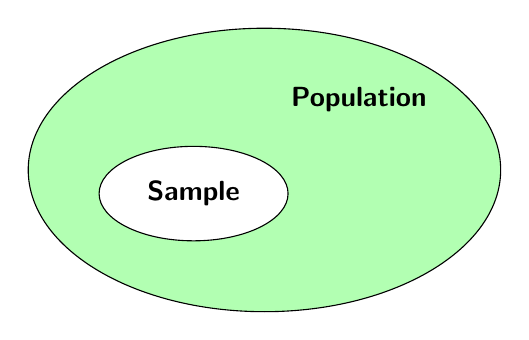
\begin{tikzpicture}[scale=0.6]
\draw [fill=green!30] (0,0) ellipse (5cm and 3cm);
\node at (2,1.5) {\textbf{Population}};
\draw [fill=white] (-1.5,-0.5) ellipse (2cm and 1cm);
\node at (-1.5,-0.5) {\textbf{Sample}};
\end{tikzpicture}
\end{center}

\begin{example}
Identify the population and the sample of each of the following.
\begin{enumerate}[(a)]
    \item 100 people at the mall were surveyed as to whether or not they like the mall.
    \item Doctors analyzed the MRIs of 38 professional boxers for possible brain injury.
\end{enumerate}
\end{example}

\subsection*{Statistical vs. Practical significance}


As we progress, keep in mind that chance and randomness are always a factor in the study of statistics, and things are not as foolproof as they are in other math courses.	\newline\\	

% A big part of interpreting and drawing conclusions from statistical results is to determine if they are considered statistically significant.	\newline\\	


\begin{tcolorbox}[colframe=green!60!black,title=\textbf{Statistically Significant}]
\textbf{Statistically significant} results are those that are not likely obtained by chance.
\end{tcolorbox}

\begin{example}
Determine if each outcome would be considered statistically significant.
\begin{enumerate}[(a)]
    \item Flipping a coin 100 times and getting tails 94 times.		
    \item Flipping a coin 100 times and getting tails 53 times.
\end{enumerate}
\end{example}

\begin{tcolorbox}[colframe=green!60!black,title=\textbf{Practically Significant}]
\textbf{Practically significant} results are those that are useful in the real world.
\end{tcolorbox}
\vspace{8pt}	

% For instance, an SAT prep course might have statistically significant results (e.g. a high percentage of people did improve their scores), but if the improvement is small, such as 20 points, the results might not be practical enough to purchase it.


\subsection*{Qualitative and Quantitative Data}

\begin{tcolorbox}[colframe=green!60!black,title=\textbf{Qualitative Data}]
\textbf{Qualitative data} (a.k.a. \textit{categorical data}) is data that is based on some quality or characteristic.
\end{tcolorbox}
\vspace{6pt} 
For instance:
\begin{itemize}
	\item Your name
	\item Blood type
	\item Zip code
\end{itemize} 



\begin{tcolorbox}[colframe=green!60!black,title=\textbf{Quantitative Data}]
\textbf{Quantitative data} is data that is based on some \emph{\underline{measurable}} numeric value.
\end{tcolorbox}
\vspace{6pt} 
Not all numeric data is quantitative.	\newline\\	

If two data values can be added together (or subtracted) to produce {\color{blue}\textbf{meaningful}} results, then the data is quantitative. Else, it is qualitative.

\begin{example}
Determine if each of the following represents qualitative or quantitative data.
\begin{enumerate}[(a)]
    \item The amount of water a household uses in a month. 	
    \item Each student's favorite color in a statistics class.
    \item Social security numbers.
    \item How much money you have on you right now. 
\end{enumerate}
\end{example}

\subsection*{Discrete vs. Continuous Data}


Within the realm of quantitative data, there are two types: discrete and continuous.	\newline\\	
\begin{center}
\tikzstyle{level 1} = [level distance = 3cm, sibling distance = 10cm]
\tikzstyle{level 2} = [level distance = 3cm, sibling distance = 1.25cm]
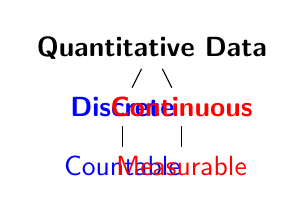
\begin{tikzpicture}[scale=0.5]
	\node {\textbf{Quantitative Data}}
		child {node {\color{blue}\textbf{Discrete}}
			child {node {\color{blue}Countable}}}
		child {node {\color{red}\textbf{Continuous}}
			child {node {\color{red}Measurable}}};
\end{tikzpicture}
\end{center}

\begin{example}
Determine whether each quantitative variable is discrete or continuous.
\begin{enumerate}[(a)]
    \item Number of free throws made.
    \item Time it takes to finish a book.
    \item Water pressure from a fire hose.
    \item The amount of money in a retirement account.
\end{enumerate}
\end{example}

% \section{Classify data by its level of measurement}


% In addition to qualitative and quantitative (and the quantitative variables discrete and continuous), there are 4 different levels of measurement of data.	\newline\\	
% \begin{tcolorbox}[colframe=green!20!black, colback = green!30!white,title=\textbf{Nominal Level of Data}]
% The \textbf{nominal level of measurement} involves only categorical data; the data can't be arranged in a meaningful order.
% \end{tcolorbox}


% \begin{tcolorbox}[colframe=green!20!black, colback = green!30!white,title=\textbf{Ordinal Level of Data}]
% The \textbf{ordinal level of measurement} involves data that can be arranged in a meaningful order, but differences in data values can't be found or are meaningless.
% \end{tcolorbox}

% \begin{tcolorbox}[colframe=green!20!black, colback = green!30!white,title=\textbf{Interval Level of Data}]
% The \textbf{interval level of measurement} involves data that can be arranged in a meaningful order, the differences are meaningful, but ratios are meaningless.
% \end{tcolorbox}
% \vspace{10pt}	
% \emph{Note}: With interval level of measurement, there is no natural zero starting point and negative values can exist.


% \begin{tcolorbox}[colframe=green!20!black, colback = green!30!white,title=\textbf{Ratio Level of Data}]
% The \textbf{ratio level of measurement} involves data that can be arranged in a meaningful order, the differences are meaningful, but there is a natural zero starting point and ratios are meaningful.
% \end{tcolorbox}


% \begin{example}
% Classify each by level of measurement.	\newline\\
% (a) \quad Top 10 cities to live in. 	\quad  Ordinal \newline\\ 
% (b) \quad Amount of coffee in a cup. \quad  Ratio \newline\\ 
% (c) \quad Room temperature (in degrees Celsius). \quad  Interval \newline\\ 
% (d) \quad Your blood type. \quad  Nominal
% \end{example}


\subsection*{Observational study vs. Experiment}

\begin{tcolorbox}[colframe=green!60!black,title=\textbf{Observational Study}]
An \textbf{observational study} is a method to obtain data in which the collector (researcher) does not get involved.
\end{tcolorbox}
\vspace{8pt} 

Observational studies try to take as much of a \textit{hands-off approach} as possible. \newline\\	
Researcher does not interject themselves into the study. 


\begin{tcolorbox}[colframe=green!60!black,title=\textbf{Experiment}]
In an \textbf{experiment}, the researcher 
\begin{itemize}
    \item divides subjects into groups
    \item applies a treatment to 1 group
    \item notes the effects (if any) between the groups
\end{itemize}
\end{tcolorbox}
\vspace{8pt}	
Typically divided into 2 groups:
\begin{itemize}
	\item \textbf{Experimental}: group that receives the treatment.	
	\item \textbf{Control}: group that either does not receive treatment or receives a ``fake" treatment (such as a \textit{placebo}).
\end{itemize}

\begin{example}
Classify each as either an observational study or an experiment.
\begin{enumerate}[(a)]
    \item A survey of 1,000 people is conducted to determine the best dog breed.
    \item 83 patients are given a new anxiety medication and 75 patients are given a sugar pill.
\end{enumerate}
\end{example}

\subsection*{Sampling Methods}

There are various ways in which to take samples, and depending on the research, one might be more appropriate than another.	\newline\\	

However, keep in mind that {\color{blue}\textbf{good sampling incorporates randomness into the process.}}

\begin{itemize}
	\item \textbf{Random sampling}
	\begin{itemize}
		\item Each member of the population has an equal chance of being selected.
	\end{itemize}	\vspace{10pt}
	\item \textbf{Stratified sampling}
	\begin{itemize}
		\item Divide the population into non-overlapping groups (\textit{strata}).
		\item Randomly sample from each group.
		\item (Some from all)
	\end{itemize}
\end{itemize}


\begin{itemize}
	\item \textbf{Cluster sampling}
	\begin{itemize}
		\item Divide the population into non-overlapping groups.
		\item Randomly pick groups and obtain information from everyone in those groups.
		\item (All from some)
	\end{itemize}	\vspace{10pt}
	\item \textbf{Systematic sampling}
	\begin{itemize}
		\item Subjects are placed in some order.
		\item Pick a random starting value ($n$).
		\item Pick a random value to count by ($k$).
		\item Starting at $n$, take every $k$\textsuperscript{th} subject thereafter.
	\end{itemize}
\end{itemize}

\begin{itemize}
	\item \textbf{Convenience sampling}
	\begin{itemize}
		\item Subjects select themselves.
		\item Results are easily obtained.
		\item Least effective and desirable method.
		\item Also known as a \textit{voluntary response sample}.
	\end{itemize}
\end{itemize}

\begin{example}
Classify each by the sampling method used.
\begin{enumerate}[(a)]
    \item An achievement test is given to all 9\textsuperscript{th} and 12\textsuperscript{th} grade students at a local high school.
    \item A radio station asks listeners to call in with their opinion on a political issue.
    \item A quality control manager selects the 5\textsuperscript{th} circuit board on an assembly line and then selects every 14\textsuperscript{th} circuit board after that.	
    \item 10 seniors, 12 juniors, 13 sophomores, and 10 freshmen are asked to name their favorite food.
    \item 10 names are drawn out of a hat containing 50 names.
\end{enumerate}
\end{example}

% \section{Examine various types of observational studies and experiments}


% \begin{itemize}
% 	\item Cross-Sectional
% 		\begin{itemize}
% 		\item Data is collected and observed at one point in time. 
% 		\end{itemize}
% 	\item Retrospective
% 		\begin{itemize}
% 		\item Collecting data from past events 
% 		\end{itemize}
% 	\item Longitudinal
% 		\begin{itemize}
% 		\item Collect future data from groups with common factors.
% 		\end{itemize}
% \end{itemize}


% \begin{itemize}
% 	\item Blind
% 	\begin{itemize}
% 		\item Researcher knows what group (experimental vs. control) the subject is in, but the subject doesn't.
% 	\end{itemize}
% 	\item Double-blind
% 	\begin{itemize}
% 		\item Neither the researcher nor the subject knows which group the subject is in; a third party knows but does not reveal. 
% 	\end{itemize}
% \end{itemize}


% Good experiments will take the following into consideration:
% \begin{itemize}
% 	\item Subjects are assigned to different groups through random selection.
% 	\item Experiments are performed on more than one subject (known as \textit{replication}).
% 	\item The sample size is large enough to see the true nature of the effects.
% 	\item Researchers will control the effects of the variables using such techinques as blinding.
% \end{itemize}


% \section{Examine errors and other issues in sampling}

% No matter how well-designed a study or experiment can be, there is always room for error.
% \begin{itemize}
% 	\item \textbf{Sampling error}
% 	\begin{itemize}
% 		\item The difference between the sample result and the true population result.
% 	\end{itemize}
% 	\item \textbf{Nonsampling error}
% 	\begin{itemize}
% 		\item Sample data isn't collected, recorded, or analyzed correctly.
% 	\end{itemize}
% 	\item \textbf{Not using randomness}
% 	\begin{itemize}
% 		\item Avoid (or take with healthy dose of skepticism) sample data that does not have some component of randomness to it, such as a convenience sample.
% 	\end{itemize}
% \end{itemize}

% \begin{itemize}
% 	\item \textbf{Small sample sizes}
% 	\begin{itemize}
% 		\item Make sure the sample size is large enough to include a variety of data regarding the population.
% 		\item More info on this later in the course.
% 	\end{itemize}
% 	\item \textbf{Non-responses}
% 	\begin{itemize}
% 		\item When someone refuses to respond to a question or is unavailable.
% 		\item How are missing values handled? As n/a? As 0?
% 	\end{itemize}
% 	\item \textbf{Loaded question}
% 	\begin{itemize}
% 		\item A question worded in order to mislead or elicit a desired response.
% 	\end{itemize}
% \end{itemize}

% \begin{example}
% Which of the following is a loaded question?	\newline\\
% (1) \quad ``Should the fire department receive additional funding for new equipment?"	\newline\\
% (2) \quad ``Should taxpayers be responsible for new fire department equipment?"			\newline\\ 

% Statement (2) is a loaded question.
% \end{example}

\end{document}